\documentclass[11pt,a4paper]{report}

\usepackage[margin=2.2cm]{geometry}
\usepackage{amsmath,amssymb,amsthm}
\usepackage{graphicx}
\usepackage{booktabs}
\usepackage{longtable}
\usepackage{array}
\usepackage{float}
\usepackage{xcolor}
\usepackage{enumitem}
\usepackage{microtype}
\usepackage{fancyhdr}
\usepackage[hidelinks,
    pdftitle={GWLab: Gravitational-Wave Matched Filtering and Bayesian Parameter-Estimation Laboratory},
    pdfauthor={SOUMITRA PHARIKAL},
    pdfsubject={Gravitational-Wave Data Analysis, Matched Filtering, Bayesian Inference, GW150914 Validation}
]{hyperref}

\sloppy

\definecolor{accent}{HTML}{1D4ED8}
\definecolor{muted}{HTML}{4B5563}
\definecolor{calloutbg}{HTML}{F8FAFC}

\pagestyle{fancy}
\fancyhf{}
\fancyhead[L]{\small\textcolor{muted}{GWLab Scientific Monograph}}
\fancyhead[R]{\small\textcolor{muted}{\leftmark}}
\fancyfoot[C]{\small\thepage}
\renewcommand{\headrulewidth}{0.4pt}

\newtheorem{remark}{Scientific Qualification}

\title{
    \vspace{-1cm}
    {\Large\textbf{GWLab: Gravitational-Wave Matched Filtering and Bayesian Parameter-Estimation Laboratory}}\\[0.6em]
    {\large A Complete Mathematical, Algorithmic, and Software Monograph}
}
\author{\textbf{SOUMITRA PHARIKAL}\\[0.25em]
\normalsize Independent Scientific Computing Project}
\date{November 26, 2026}

\begin{document}

\maketitle
\thispagestyle{empty}

\begin{abstract}
\textbf{GWLab} is a reproducible scientific computing and interactive web laboratory for compact binary coalescence (CBC) gravitational-wave signal modeling, noise spectral estimation, matched filtering, and Bayesian nested-sampling parameter estimation. This monograph develops the complete mathematical and algorithmic foundations of the system from first principles for readers familiar with undergraduate physics and mathematics. Starting from binary inspiral dynamics and the stationary-phase \texttt{TaylorF2} $3.5\mathrm{PN}$ frequency-domain waveform, we derive the discrete Fourier and one-sided power spectral density (PSD) conventions, synthetic colored Gaussian noise generation, Welch periodogram estimation with overlap-variance inflation, the noise-weighted inner product and matched-filter signal-to-noise ratio (SNR), the normalized active-band Whittle Gaussian log-likelihood, and nested-sampling Bayesian inference including circular phase statistics.

Every equation, physical constant, and post-Newtonian coefficient in this document is verified directly against the implemented Python scientific engine (\texttt{src/gw\_inference/}), the FastAPI service (\texttt{src/gwlab/api/}), and the Next.js~\texttt{16.4.6} frontend (\texttt{frontend/}). Under the frozen synthetic benchmark ($4.0\,\mathrm{s}$ segment at $2048\,\mathrm{Hz}$, active band $[20, 512]\,\mathrm{Hz}$, custom analytical aLIGO-like PSD proxy), the matched filter achieves optimal template SNR $\rho_{\mathrm{opt}} = 45.3153$, the saved synthetic benchmark posterior (random seed $8101$) yields $\ln Z = 201646.1413 \pm 0.2374\,\mathrm{nats}$ across $11{,}951$ weighted samples (with $38.57\%$ of posterior mass in the upper $1\%$ of the symmetric-mass-ratio prior and circular coalescence-phase mean $\bar{\phi}_c = 0.0538\,\mathrm{rad}$, $\bar{R} = 0.6991$), and the two-seed evidence sensitivity comparison ($8101$ vs.\ $8201$) records $|\Delta \ln Z| = 2.9720\,\mathrm{nats}$ (ratio $8.92$). All scientific qualifications, software architecture boundaries, and validation results ($517/517$ synthetic backend tests, $86\%$ \texttt{src/gwlab/} coverage, $21/21$ Playwright checks) are documented alongside an independent known-event external validation on public GWOSC \textbf{GW150914} H1/L1 strain ($32\,\mathrm{s}$, $4096\,\mathrm{Hz}$ downsampled to $2048\,\mathrm{Hz}$), where a fixed, non-optimized \texttt{TaylorF2} inspiral template applied to a known event recovers coherent matched-filter peaks near the catalog GPS time ($8.94$ in H1 at $+71.8\,\mathrm{ms}$ and $5.55$ in L1 at $+61.0\,\mathrm{ms}$). Full Bayesian parameter-estimation or generalization validation on real data has not been performed.
\end{abstract}

\tableofcontents
\clearpage

%==============================================================================
\chapter{Introduction}
%==============================================================================

\section{Gravitational Waves and Compact Binary Coalescence}
General relativity predicts that accelerating asymmetric mass distributions radiate ripples in spacetime curvature---gravitational waves---propagating at the speed of light $c$. In the weak-field, far-zone limit, a gravitational wave passing a terrestrial laser interferometer induces a dimensionless fractional arm-length change, or \emph{strain},
\begin{equation}
h(t) = \frac{\Delta L(t)}{L},
\end{equation}
typically of order $10^{-21}$ or smaller for astrophysical sources at hundreds of megaparsecs.

Among the most informative gravitational-wave sources are \emph{compact binary coalescences} (CBCs): pairs of neutron stars or black holes orbiting each other while losing energy and angular momentum to gravitational radiation. As energy is carried away, the orbital separation shrinks and the orbital frequency increases, producing a characteristic ``chirp'' signal whose amplitude and frequency rise monotonically through three physical regimes:
\begin{enumerate}[leftmargin=1.5em]
    \item \textbf{Inspiral:} The two bodies are well separated ($v/c \ll 1$) and spiral inward adiabatically over many orbits. The waveform is accurately described by post-Newtonian (PN) perturbation theory.
    \item \textbf{Merger:} Relativistic strong-field gravity dominates as the bodies plunge and form a single perturbed remnant.
    \item \textbf{Ringdown:} The remnant settles into a stationary Kerr black hole via damped quasinormal oscillations.
\end{enumerate}
For high-mass or short-band educational benchmarks, the inspiral phase up to the innermost stable circular orbit (ISCO) already encodes the binary's mass scale, mass ratio, arrival time, and coalescence phase.

\section{Detector Signals and the Data-Analysis Problem}
An idealized single-detector time series $d(t)$ is modeled as the sum of an astrophysical gravitational-wave signal $h(t; \theta)$ parameterized by $\theta$ and additive detector noise $n(t)$:
\begin{equation}
d(t) = h(t; \theta) + n(t).
\end{equation}
Because detector noise varies by orders of magnitude across frequency---dominated by seismic and suspension noise at low frequencies, thermal noise in the middle band, and laser shot noise at high frequencies---a gravitational-wave signal that is completely buried in raw time-domain noise can still be detected and characterized if the data are weighted inversely by the noise power at each frequency.

The central data-analysis problem has two coupled parts:
\begin{enumerate}[leftmargin=1.5em]
    \item \textbf{Detection (Matched Filtering):} Given a template waveform $h(t; \theta)$, correlate it against the noise-weighted data across arrival times to maximize the signal-to-noise ratio (SNR).
    \item \textbf{Parameter Estimation (Bayesian Inference):} Given a prior distribution $\pi(\theta)$ and a noise-derived likelihood $\mathcal{L}(d \mid \theta)$, compute the posterior probability distribution $p(\theta \mid d)$ and the Bayesian evidence $Z = \int \mathcal{L}(d \mid \theta)\,\pi(\theta)\,d\theta$.
\end{enumerate}

\section{Design Philosophy of GWLab}
GWLab separates deterministic numerical physics from interactive presentation (Figure~\ref{fig:pipeline}). Its design enforces three boundaries:
\begin{itemize}[leftmargin=1.5em]
    \item \textbf{Controlled Synthetic Benchmarking:} Interactive waveform, noise, and matched-filter tools operate on deterministic synthetic data using a custom, regularized analytical PSD proxy (\texttt{aligo\_representative}), not live or official LIGO strain/sensitivity curves.
    \item \textbf{Convention Unification:} Waveform normalization, discrete Fourier transforms, Welch PSD estimation, matched-filter SNR, and the Whittle log-likelihood share a single audited set of mathematical conventions.
    \item \textbf{Read-Only Posterior Archives:} Stochastic nested-sampling runs are expensive and require strict seed and budget governance; therefore, the web application never launches a live sampler and instead inspects frozen, provenance-tracked posterior and evidence archives.
\end{itemize}

\begin{figure}[H]
    \centering
    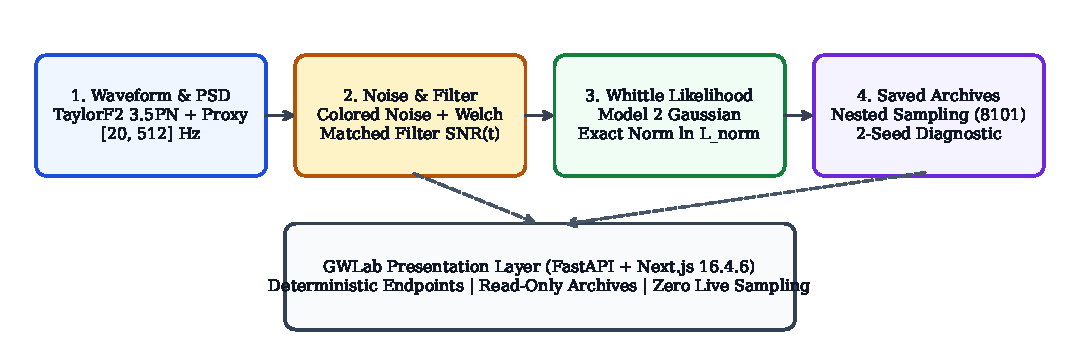
\includegraphics[width=0.98\textwidth]{figures/fig0_architecture_pipeline.pdf}
    \caption{End-to-end GWLab scientific and software architecture. Deterministic waveform, noise, and matched-filtering calculations run in real time via FastAPI over \texttt{src/gw\_inference/}, while Bayesian posterior and multi-seed evidence views read strictly from frozen archives.}
    \label{fig:pipeline}
\end{figure}

%==============================================================================
\chapter{Binary Dynamics}
%==============================================================================

\section{Mass Parameterizations}
Consider a non-spinning binary of point-like compact objects with detector-frame component masses $m_1 \ge m_2 > 0$ (in solar masses $M_\odot$ or SI kilograms via $M_\odot = 1.9884099 \times 10^{30}\,\mathrm{kg}$). Three derived mass combinations govern inspiral dynamics:
\begin{align}
M &= m_1 + m_2 \qquad &&\text{(total mass)}, \\
\eta &= \frac{m_1 m_2}{M^2} \in (0, 0.25] \qquad &&\text{(symmetric mass ratio)}, \\
\mathcal{M}_c &= M\,\eta^{3/5} = \frac{(m_1 m_2)^{3/5}}{(m_1 + m_2)^{1/5}} \qquad &&\text{(chirp mass)}.
\end{align}
The symmetric mass ratio $\eta$ attains its maximum $\eta = 0.25$ for an equal-mass binary ($m_1 = m_2$) and decreases toward $0$ in the extreme-mass-ratio limit ($m_2 \ll m_1$). Note that $\mathcal{M}_c$ has units of mass ($M_\odot$ or $\mathrm{kg}$), while $\eta$ is dimensionless.

\subsection{Inverting $(\mathcal{M}_c, \eta)$ to Component Masses}
Bayesian samplers often sample in $(\mathcal{M}_c, \eta)$ because $\mathcal{M}_c$ is constrained much more tightly by the inspiral phase than individual masses. Given $(\mathcal{M}_c, \eta)$ with $\eta \in (0, 0.25]$, we recover $M = \mathcal{M}_c\,\eta^{-3/5}$. Since $m_1 + m_2 = M$ and $m_1 m_2 = \eta M^2$, $m_1$ and $m_2$ are roots of the quadratic $m^2 - M m + \eta M^2 = 0$:
\begin{equation}
m_{1,2} = \frac{M}{2}\left(1 \pm \sqrt{1 - 4\eta}\right),
\end{equation}
with mass ratio $q = m_1 / m_2 \ge 1$. Notice that as $\eta \to 0.25$, $\sqrt{1 - 4\eta}$ has an infinite derivative with respect to $\eta$, making equal-mass boundaries geometrically sharp in $(\mathcal{M}_c, \eta)$ coordinates.

\section{Orbital and Gravitational-Wave Frequency Evolution}
In Newtonian gravity, a circular binary of total mass $M$ and orbital separation $r$ satisfies Kepler's third law,
\begin{equation}
\Omega_{\mathrm{orb}}^2 = \frac{G M}{r^3}, \qquad f_{\mathrm{orb}} = \frac{\Omega_{\mathrm{orb}}}{2\pi}.
\end{equation}
Because gravitational radiation is quadrupolar (invariant under a $180^\circ$ rotation of a symmetric orbit), the dominant gravitational-wave frequency is twice the orbital frequency:
\begin{equation}
f = 2 f_{\mathrm{orb}} = \frac{1}{\pi}\sqrt{\frac{G M}{r^3}}.
\end{equation}
In the quadrupole approximation~\cite{Finn1992,CutlerFlanagan1994}, the binary loses orbital energy $E_{\mathrm{orb}} = -G m_1 m_2 / (2r)$ at luminosity
\begin{equation}
\mathcal{L}_{\mathrm{GW}} = -\frac{dE_{\mathrm{orb}}}{dt} = \frac{32}{5}\frac{G^4}{c^5}\frac{m_1^2 m_2^2 M}{r^5}.
\end{equation}
Using $r = (G M)^{1/3} (\pi f)^{-2/3}$ to eliminate $r$ yields the leading-order frequency evolution (chirp equation):
\begin{equation}
\frac{df}{dt} = \frac{96}{5}\,\pi^{8/3}\left(\frac{G \mathcal{M}_c}{c^3}\right)^{5/3} f^{11/3}.
\end{equation}
Crucially, the leading-order inspiral rate depends on the masses \emph{only} through the chirp mass $\mathcal{M}_c$. Integrating $dt/df$ from frequency $f$ to coalescence ($f \to \infty$) gives the Newtonian time to coalescence:
\begin{equation}
\tau_0(f) = \frac{5}{256}\left(\frac{G \mathcal{M}_c}{c^3}\right)^{-5/3} (\pi f)^{-8/3}.
\end{equation}

\section{Innermost Stable Circular Orbit (ISCO)}
The inspiral approximation breaks down once the binary reaches the last stable circular orbit. For a Schwarzschild test-mass effective potential, this occurs at $r_{\mathrm{ISCO}} = 6 G M / c^2$, corresponding to gravitational-wave frequency
\begin{equation}
f_{\mathrm{ISCO}} = \frac{c^3}{6^{3/2}\,\pi G M} = \frac{C_{\mathrm{ISCO}}}{M / M_\odot},
\end{equation}
where GWLab uses the frozen specification constant $C_{\mathrm{ISCO}} = 4397.17\,\mathrm{Hz}\cdot M_\odot$ (\texttt{src/gw\_inference/constants.py}).

\subsection{Worked Example: Benchmark Binary}
For GWLab's reference injection ($\mathcal{M}_c = 28.095556\,M_\odot$, $\eta = 0.247101$, $d_L = 410.0\,\mathrm{Mpc}$):
\begin{enumerate}[leftmargin=1.5em]
    \item Total mass: $M = 28.095556 \times (0.247101)^{-3/5} \approx 64.611\,M_\odot$.
    \item Component masses: $\sqrt{1 - 4\eta} \approx 0.1077$, giving $m_1 \approx 35.78\,M_\odot$ and $m_2 \approx 28.83\,M_\odot$ ($q \approx 1.24$).
    \item Schwarzschild ISCO frequency: $f_{\mathrm{ISCO}} = 4397.17 / 64.611 \approx 68.06\,\mathrm{Hz}$.
\end{enumerate}
Because $f_{\mathrm{ISCO}} \approx 68.06\,\mathrm{Hz}$ lies well below the upper analysis cutoff $f_{\mathrm{end}} = 512\,\mathrm{Hz}$, the waveform terminates at $f_{\mathrm{term}} = \min(f_{\mathrm{end}}, f_{\mathrm{ISCO}}) = 68.06\,\mathrm{Hz}$, while the likelihood still sums over the full static active band $[20, 512]\,\mathrm{Hz}$.

%==============================================================================
\chapter{Waveform Modeling: TaylorF2 3.5PN}
%==============================================================================

\section{Stationary-Phase Approximation (SPA)}
In the time domain, an adiabatic inspiral waveform has the form $h(t) = A(t)\cos\Phi(t)$, where $A(t)$ varies slowly compared to the rapidly oscillating phase $\Phi(t)$. Its Fourier transform is
\begin{equation}
\tilde{h}(f) = \int_{-\infty}^{\infty} A(t)\,\frac{e^{i\Phi(t)} + e^{-i\Phi(t)}}{2}\,e^{-i2\pi f t}\,dt.
\end{equation}
For $f > 0$, the $e^{+i(\Phi(t) - 2\pi f t)}$ term has no stationary point when $\dot{\Phi}(t) > 0$, while the $e^{-i(\Phi(t) + 2\pi f t)}$... Wait—with the sign convention $\tilde{h}(f) = \int h(t) e^{-i2\pi f t}\,dt$ and $\dot{\Phi}(t) = 2\pi f(t) > 0$, the stationary point $t_*(f)$ occurs in the $e^{+i\Phi(t) - i2\pi f t}$ integral where $\dot{\Phi}(t_*) = 2\pi f$. Expanding $\Phi(t) - 2\pi f t \approx \Phi(t_*) - 2\pi f t_* + \frac{1}{2}\ddot{\Phi}(t_*)(t - t_*)^2$ and evaluating the Fresnel Gaussian integral $\int_{-\infty}^{\infty} e^{i \frac{1}{2}\ddot{\Phi}(t_*)\delta t^2}\,d(\delta t) = \sqrt{2\pi / \ddot{\Phi}(t_*)}\,e^{i\pi/4}$ gives the restricted frequency-domain waveform~\cite{SathyaprakashDhurandhar1991,Buonanno2009}:
\begin{equation}
\tilde{h}(f) = \mathcal{A}(f)\,e^{-i\Psi(f)}, \qquad f \in (0, f_{\mathrm{term}}].
\end{equation}

\section{Restricted Newtonian Amplitude and Dimensional Verification}
In the restricted approximation, higher PN amplitude corrections are neglected and only the leading quadrupolar amplitude is retained:
\begin{equation}
\mathcal{A}(f) = A_{\mathrm{const}}\,f^{-7/6}, \qquad A_{\mathrm{const}} = \sqrt{\frac{5}{24}}\,\pi^{-2/3}\,\frac{c}{d_L}\left(\frac{G \mathcal{M}_c}{c^3}\right)^{5/6}.
\end{equation}
We check SI dimensions explicitly (as verified in \texttt{taylorf2\_amplitude\_prefactor} in \texttt{src/gw\_inference/waveform.py}):
\begin{itemize}[leftmargin=1.5em]
    \item $[c / d_L] = (\mathrm{m}\cdot\mathrm{s}^{-1}) / \mathrm{m} = \mathrm{s}^{-1}$.
    \item $[G \mathcal{M}_c / c^3] = (\mathrm{m}^3\,\mathrm{kg}^{-1}\,\mathrm{s}^{-2})(\mathrm{kg}) / (\mathrm{m}^3\,\mathrm{s}^{-3}) = \mathrm{s}$.
    \item $[A_{\mathrm{const}}] = \mathrm{s}^{-1} \cdot \mathrm{s}^{5/6} = \mathrm{s}^{-1/6}$.
    \item $[f^{-7/6}] = (\mathrm{s}^{-1})^{-7/6} = \mathrm{s}^{7/6}$.
    \item $[\mathcal{A}(f)] = \mathrm{s}^{-1/6}\,\mathrm{s}^{7/6} = \mathrm{s} = \mathrm{Hz}^{-1}$, matching the time-scaled Fourier transform $\tilde{h}(f) = \int h(t) e^{-i2\pi f t}\,dt$ of a dimensionless strain $h(t)$.
\end{itemize}

\section{Complete Implemented 3.5PN Fourier Phase}
In terms of the dimensionless post-Newtonian orbital velocity parameter
\begin{equation}
v(f) = \left(\frac{\pi G M f}{c^3}\right)^{1/3} = \left(\frac{\pi G \mathcal{M}_c f}{c^3}\right)^{1/3} \eta^{-1/5},
\end{equation}
GWLab implements the \texttt{TaylorF2} Fourier phase (\texttt{taylorf2\_35pn\_phase} and \texttt{apply\_coalescence\_time\_shift} in \texttt{src/gw\_inference/waveform.py}) as
\begin{equation}
\Psi(f) = 2\pi f t_c - \phi_c - \frac{\pi}{4} + \frac{3}{128\,\eta\,v^5}\sum_{k=0}^{7} \alpha_k(\eta, v)\,v^k,
\end{equation}
where $t_c$ is the coalescence arrival time (in seconds), $\phi_c$ is the coalescence phase (in radians), and $\gamma_E = 0.5772156649\dots$ is the Euler--Mascheroni constant. Verified line-by-line against \texttt{src/gw\_inference/waveform.py} (lines 220--241) and standard PN literature~\cite{Buonanno2009}, the implemented coefficients $\alpha_0$ through $\alpha_7$ are:
\begin{align}
\alpha_0 &= 1, \\
\alpha_1 &= 0 \qquad \text{(no $0.5\mathrm{PN}$ dipole radiation in GR)}, \\
\alpha_2 &= \frac{3715}{756} + \frac{55}{9}\eta \qquad \text{($1.0\mathrm{PN}$)}, \\
\alpha_3 &= -16\pi \qquad \text{($1.5\mathrm{PN}$ leading tail)}, \\
\alpha_4 &= \frac{15293365}{508032} + \frac{27145}{504}\eta + \frac{3085}{72}\eta^2 \qquad \text{($2.0\mathrm{PN}$)}, \\
\alpha_5 &= \pi\left(\frac{38645}{756} - \frac{65}{9}\eta\right)\big(1 + 3\ln v\big) \qquad \text{($2.5\mathrm{PN}$ logarithmic tail)}, \\
\alpha_6 &= \frac{11583231236531}{46942156800} - \frac{6848}{21}\gamma_E - \frac{640}{3}\pi^2 + \left(-\frac{15737765635}{3048192} + \frac{2255}{12}\pi^2\right)\eta \nonumber\\
         &\quad + \frac{76055}{1728}\eta^2 - \frac{127825}{1296}\eta^3 - \frac{6848}{21}\ln(4v) \qquad \text{($3.0\mathrm{PN}$)}, \\
\alpha_7 &= \pi\left(\frac{77096675}{254016} + \frac{378515}{1512}\eta - \frac{74045}{756}\eta^2\right) \qquad \text{($3.5\mathrm{PN}$)}.
\end{align}
All coefficients are dimensionless, so $\Psi(f)$ is in radians. Because the waveform is real in the time domain, negative frequencies satisfy Hermitian symmetry $\tilde{h}(-f) = \tilde{h}^*(f)$, while GWLab evaluates waveforms exclusively on the non-negative physical frequency grid $f_k \ge 0$ with $h(f_k) = 0$ outside $(0, f_{\mathrm{term}}]$.

%==============================================================================
\chapter{Fourier Analysis and Discrete Conventions}
%==============================================================================

\section{Sampling, Frequency Resolution, and DFT Normalization}
A continuous time series $x(t)$ sampled at rate $f_s = 1/\Delta t$ over duration $T = N \Delta t$ produces $N$ discrete samples $x_j = x(j\Delta t)$ for $j = 0, 1, \dots, N-1$. In the frozen benchmark configuration, $T = 4.0\,\mathrm{s}$ and $f_s = 2048.0\,\mathrm{Hz}$, giving $N = 8192$ samples, frequency bin spacing $\Delta f = 1/T = 0.25\,\mathrm{Hz}$, and Nyquist frequency $f_{\mathrm{Nyq}} = f_s / 2 = 1024.0\,\mathrm{Hz}$.

To match continuous-time Fourier units ($[\tilde{x}(f)] = [x]\cdot\mathrm{s}$), GWLab defines the time-scaled forward discrete Fourier transform (\texttt{continuous\_rfft} in \texttt{src/gw\_inference/conventions.py}) as
\begin{equation}
\tilde{x}(f_k) = \Delta t \sum_{j=0}^{N-1} x_j\,e^{-i 2\pi j k / N}, \qquad f_k = k\,\Delta f, \quad k = 0, 1, \dots, \frac{N}{2},
\end{equation}
and the corresponding inverse transform as
\begin{equation}
x_j = \Delta f \sum_{k=0}^{N-1} \tilde{x}(f_k)\,e^{+i 2\pi j k / N}.
\end{equation}
Because $\Delta t \cdot \Delta f = 1/N$, the inverse recovers $x_j$ identically.

\section{Parseval's Theorem and One-Sided Spectra}
With the $\Delta t$ scaling above, Parseval's energy identity holds in direct analogy to the continuous integral:
\begin{equation}
\Delta t \sum_{j=0}^{N-1} x_j^2 = \Delta f \sum_{k=0}^{N-1} |\tilde{x}(f_k)|^2 = \Delta f \left( |\tilde{x}(0)|^2 + |\tilde{x}(f_{\mathrm{Nyq}})|^2 + 2\sum_{k=1}^{N/2 - 1} |\tilde{x}(f_k)|^2 \right).
\end{equation}
The factor of $2$ on interior positive frequencies $1 \le k < N/2$ accounts for the conjugate-symmetric negative-frequency bins ($\tilde{x}(-f_k) = \tilde{x}^*(f_k)$) and is the exact origin of the factor of $4\,\Delta f$ (rather than $2\,\Delta f$) in the one-sided noise-weighted inner product and Whittle likelihood derived in Chapters~\ref{ch:matched_filter} and~\ref{ch:likelihood}.

%==============================================================================
\chapter{Detector Noise and Welch PSD Estimation}
%==============================================================================

\section{Stationary Gaussian Noise, PSD, and ASD}
Stationary, zero-mean Gaussian noise $n(t)$ is completely characterized in the frequency domain by its one-sided power spectral density $S_n(f)$ (units: $\mathrm{Hz}^{-1}$ for dimensionless strain), defined for $f > 0$ via
\begin{equation}
\mathbb{E}\!\left[\tilde{n}^*(f)\,\tilde{n}(f')\right] = \frac{1}{2} S_n(f)\,\delta(f - f').
\end{equation}
In discrete frequency bins of width $\Delta f = 1/T$, the Dirac delta becomes $\delta(f - f') \to \delta_{kk'} / \Delta f$, so
\begin{equation}
\mathbb{E}\!\left[|\tilde{n}(f_k)|^2\right] = \frac{S_n(f_k)}{2\,\Delta f} = \frac{N\,S_n(f_k)}{2\,f_s}, \qquad 1 \le k < N/2.
\end{equation}
Because $\tilde{n}(f_k) = \operatorname{Re}\tilde{n}(f_k) + i\operatorname{Im}\tilde{n}(f_k)$ is a proper complex circular Gaussian variable, its real and imaginary parts are independent zero-mean real Gaussians with equal variance:
\begin{equation}
\operatorname{Var}\!\big(\operatorname{Re}\tilde{n}(f_k)\big) = \operatorname{Var}\!\big(\operatorname{Im}\tilde{n}(f_k)\big) = \frac{S_n(f_k)}{4\,\Delta f} = \frac{N\,S_n(f_k)}{4\,f_s}.
\end{equation}
The amplitude spectral density (ASD) is $\mathrm{ASD}(f) = \sqrt{S_n(f)}$ in $\mathrm{Hz}^{-1/2}$, allowing direct visual comparison of noise floors across frequency.

\section{Analytical PSD Proxy Qualification}
\begin{remark}
The default \texttt{aligo\_representative} model in GWLab is a \textbf{custom, regularized analytical aLIGO-like PSD proxy} designed for controlled numerical benchmarking. It is \textbf{not} an official Advanced LIGO design-sensitivity curve and \textbf{not} a measured LIGO Hanford (H1) spectrum.
\end{remark}
Verified directly against \texttt{analytical\_detector\_psd} in \texttt{src/gw\_inference/psd.py} (lines 1166--1177), the analytical proxy is
\begin{equation}
S_n(f) = S_0 \left[ \left(\frac{f_{\mathrm{knee}}^2}{f^2 + f_{\mathrm{reg}}^2}\right)^{\!2} + 1 + \left(\frac{f}{f_{\mathrm{high}}}\right)^{\!2} \right],
\end{equation}
with $S_0 = 1.0 \times 10^{-46}\,\mathrm{Hz}^{-1}$, $f_{\mathrm{knee}} = 35.0\,\mathrm{Hz}$, $f_{\mathrm{reg}} = 15.0\,\mathrm{Hz}$, and $f_{\mathrm{high}} = 300.0\,\mathrm{Hz}$. The regularization $f_{\mathrm{reg}}$ ensures a finite DC value $S_n(0) = S_0[(35/15)^4 + 1] \approx 30.642 \times 10^{-46}\,\mathrm{Hz}^{-1}$. A constant white-noise reference (\texttt{flat}) with $S_n(f) = S_0$ is also supported.

\section{Synthetic Colored Noise and Welch Estimation}
To synthesize deterministic colored Gaussian noise (\texttt{generate\_colored\_noise}), GWLab draws independent standard normal real and imaginary components at each interior bin $1 \le k < N/2$, scales each by $\sqrt{S_n(f_k)/(4\Delta f)}$, sets real Nyquist/DC components appropriately, and applies the inverse real FFT.

For empirical PSD estimation on an off-source stretch of duration $T_{\mathrm{obs}} = 64.0\,\mathrm{s}$, GWLab uses Welch's overlapped segmented periodogram~\cite{Welch1967}:
\begin{enumerate}[leftmargin=1.5em]
    \item Divide the series into $K$ overlapping segments of length $M = 8192$ samples ($T_{\mathrm{seg}} = 4.0\,\mathrm{s}$) with $50\%$ overlap (hop $H = M/2 = 4096$), yielding $K = 31$ segments.
    \item Multiply each segment by a symmetric midpoint Tukey window ($\alpha = 0.25$) and compute its window power normalization $S_2 = \frac{1}{M}\sum_{j=0}^{M-1} w_j^2$.
    \item Average the one-sided segment periodograms $\widehat{S}_m(f_k) = \frac{2\Delta t}{M S_2}|X_k^{(m)}|^2$ (for $1 \le k < M/2$) across all $K$ segments: $\widehat{S}_{\mathrm{Welch}}(f_k) = \frac{1}{K}\sum_{m=0}^{K-1} \widehat{S}_m(f_k)$.
\end{enumerate}
Because overlapping segments share data, the variance of $\widehat{S}_{\mathrm{Welch}}$ is inflated relative to $K$ independent segments by the all-lags overlap factor
\begin{equation}
\kappa_{\mathrm{overlap}} = 1 + 2 \sum_{\ell=1}^{\ell_{\max}} \left(1 - \frac{\ell}{K}\right) r_\ell^2, \qquad r_\ell = \frac{\sum_{j=0}^{M - \ell H - 1} w_j w_{j + \ell H}}{\sum_{j=0}^{M-1} w_j^2}.
\end{equation}
For $K = 31$, $50\%$ overlap, and $\alpha = 0.25$, GWLab obtains $\kappa_{\mathrm{overlap}} = 1.3823$ and effective degrees of freedom $\nu_{\mathrm{eff}} = 2K / \kappa_{\mathrm{overlap}} = 44.85$ (rather than $2K = 62$). Figure~\ref{fig:psd_asd} illustrates the close agreement between the synthetic Welch ASD estimate (\texttt{seed=7101}) and the analytical proxy across $[20, 512]\,\mathrm{Hz}$.

\begin{figure}[H]
    \centering
    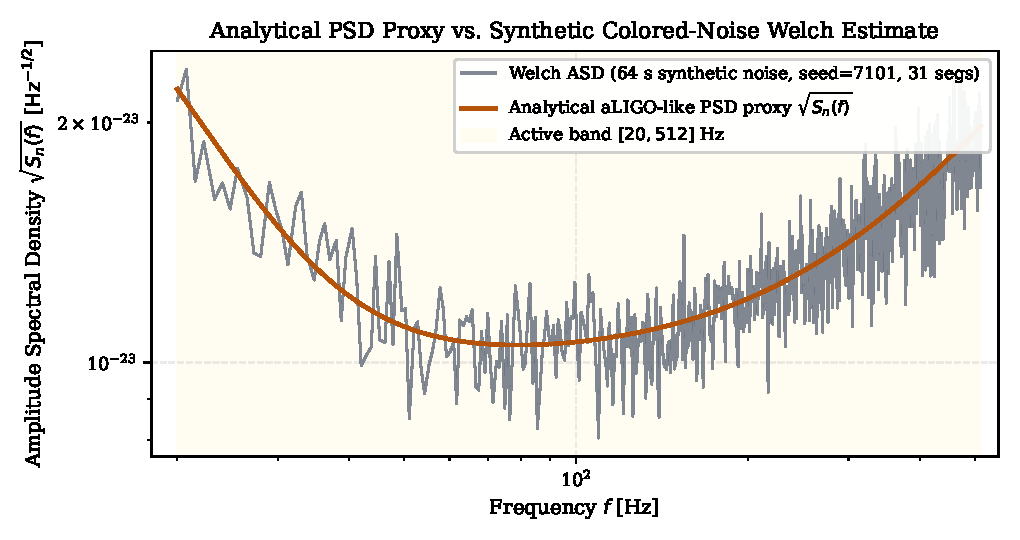
\includegraphics[width=0.92\textwidth]{figures/fig1_psd_asd.pdf}
    \caption{Analytical aLIGO-like ASD proxy $\sqrt{S_n(f)}$ (amber) versus Tukey-windowed Welch ASD estimate (gray) from a $64\,\mathrm{s}$ synthetic colored Gaussian noise realization (\texttt{seed=7101}, $31$ segments, $\alpha = 0.25$, $50\%$ overlap, $\kappa_{\mathrm{overlap}} = 1.3823$, $\nu_{\mathrm{eff}} = 44.85$).}
    \label{fig:psd_asd}
\end{figure}

%==============================================================================
\chapter{Matched Filtering}\label{ch:matched_filter}
%==============================================================================

\section{Noise-Weighted Inner Product and Optimal Filter}
Consider a real linear filter $Q(t)$ applied to data $d(t) = h(t) + n(t)$:
\begin{equation}
O = \int_{-\infty}^{\infty} \tilde{d}(f)\,\tilde{Q}^*(f)\,df = 2\operatorname{Re}\int_0^{\infty} \tilde{d}(f)\,\tilde{Q}^*(f)\,df.
\end{equation}
For signal $h$ alone, the expected output is $\mathbb{E}[O \mid h] = 2\operatorname{Re}\int_0^\infty \tilde{h}(f)\tilde{Q}^*(f)\,df$. For stationary colored noise with $\mathbb{E}[\tilde{n}^*(f)\tilde{n}(f')] = \frac{1}{2}S_n(f)\delta(f-f')$, the noise variance is $\mathbb{E}[O^2 \mid n] = \int_0^\infty S_n(f)|\tilde{Q}(f)|^2\,df$. Defining the one-sided noise-weighted inner product
\begin{equation}
\langle a \mid b \rangle = 4\operatorname{Re}\int_{f_{\min}}^{f_{\max}} \frac{\tilde{a}^*(f)\,\tilde{b}(f)}{S_n(f)}\,df \;\approx\; 4\,\Delta f \operatorname{Re}\sum_{k \in \mathcal{K}_+} \frac{\tilde{a}^*(f_k)\,\tilde{b}(f_k)}{S_n(f_k)},
\end{equation}
we can rewrite the signal-to-noise ratio $\rho = \mathbb{E}[O \mid h] / \sqrt{\mathbb{E}[O^2 \mid n]}$ as
\begin{equation}
\rho = \frac{\langle h \mid S_n Q \rangle}{\sqrt{\langle S_n Q \mid S_n Q \rangle}}.
\end{equation}
By the Cauchy--Schwarz inequality, $\rho$ is maximized when $\tilde{Q}(f) \propto \tilde{h}(f) / S_n(f)$---the \emph{Wiener matched filter}~\cite{Allen2012}, which downweights noisy frequencies and boosts sensitive bands.

\section{Template Normalization, Complex SNR, and Mismatch Loss}
Setting the template normalization to $\sigma_h = \sqrt{\langle h \mid h \rangle}$, the expected optimal SNR for a zero-mismatch signal is $\rho_{\mathrm{opt}} = \sigma_h$ (dimensionless, because $[\tilde{h}] = \mathrm{s}$, $[\Delta f] = \mathrm{s}^{-1}$, $[S_n] = \mathrm{s}$, so $\Delta f |\tilde{h}|^2 / S_n$ is dimensionless). Evaluating the matched filter across all coalescence time shifts $t_j = j\Delta t$ via inverse FFT yields the complex SNR time series:
\begin{equation}
\rho(t_j) = \frac{4\,\Delta f}{\sigma_h} \sum_{k \in \mathcal{K}_+} \frac{\tilde{d}(f_k)\,\tilde{h}_{\mathrm{tmpl}}^*(f_k)}{S_n(f_k)}\,e^{+i 2\pi f_k t_j}.
\end{equation}
Because shifting the coalescence phase $\phi_c \to \phi_c + \delta\phi$ multiplies $\rho(t_j)$ by $e^{i\delta\phi}$, taking the magnitude $|\rho(t_j)|$ analytically maximizes over unknown $\phi_c$.

Figure~\ref{fig:matched_filter} shows the synthetic benchmark (\texttt{seed=7151}, injected $t_c = 2.0\,\mathrm{s}$, $\rho_{\mathrm{opt}} = 45.3153$). A matched template ($\Delta\mathcal{M}_c = 0$) recovers peak SNR $44.28$ at $t \approx 2.0\,\mathrm{s}$ (differing from $\rho_{\mathrm{opt}}$ due to the particular synthetic noise fluctuation), whereas a $+2.5\,M_\odot$ chirp-mass mismatch dephases the template across the inspiral and drops the recovered peak SNR to $34.43$.

\begin{figure}[H]
    \centering
    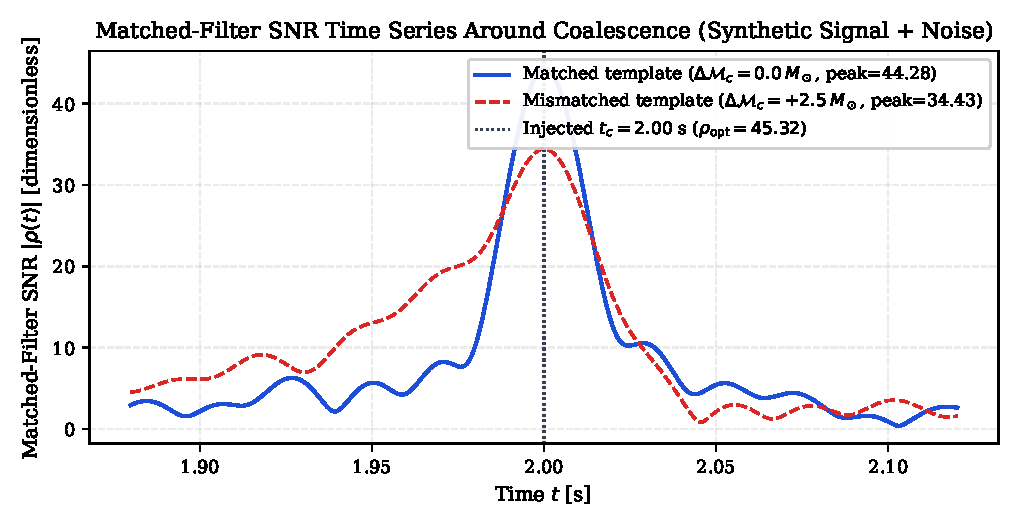
\includegraphics[width=0.92\textwidth]{figures/fig2_matched_filter_snr.pdf}
    \caption{Matched-filter SNR $|\rho(t)|$ around coalescence for synthetic injection + colored Gaussian noise (\texttt{seed=7151}, $\rho_{\mathrm{opt}} = 45.3153$). Zero template mismatch ($\Delta\mathcal{M}_c = 0$) recovers $44.28$, while $\Delta\mathcal{M}_c = +2.5\,M_\odot$ degrades the peak to $34.43$.}
    \label{fig:matched_filter}
\end{figure}

%==============================================================================
\chapter{Frequency-Domain Whittle Likelihood}\label{ch:likelihood}
%==============================================================================

\section{Derivation from Gaussian Noise Assumptions}
Given data $\tilde{d}(f_k)$ and signal model $\tilde{h}(f_k; \theta)$, the complex residual is $\tilde{r}_k(\theta) = \tilde{d}(f_k) - \tilde{h}(f_k; \theta)$. Under the hypothesis that $\theta$ is the true parameter vector, $\tilde{r}_k(\theta) = \tilde{n}(f_k)$ is stationary colored Gaussian noise.

In the Whittle approximation~\cite{Finn1992}, Fourier bins in the active positive-frequency set $\mathcal{K}_+ = \{k : 20\,\mathrm{Hz} \le f_k \le 512\,\mathrm{Hz}\}$ ($k \in [80, 2048]$, DC and Nyquist excluded) are treated as mutually independent proper complex Gaussian random variables with real and imaginary variances $\sigma_k^2 = \frac{N S_n(f_k)}{4 f_s} = \frac{S_n(f_k)}{4\Delta f}$. The joint probability density for a single bin $k$ is the product of two independent 1D Gaussians:
\begin{equation}
p\big(\tilde{r}_k \mid \theta\big) = \frac{1}{\sqrt{2\pi \sigma_k^2}} \exp\!\left(-\frac{(\operatorname{Re}\tilde{r}_k)^2}{2\sigma_k^2}\right) \cdot \frac{1}{\sqrt{2\pi \sigma_k^2}} \exp\!\left(-\frac{(\operatorname{Im}\tilde{r}_k)^2}{2\sigma_k^2}\right) = \frac{1}{2\pi \sigma_k^2}\exp\!\left(-\frac{|\tilde{r}_k|^2}{2\sigma_k^2}\right).
\end{equation}
Substituting $2\sigma_k^2 = \frac{N S_n(f_k)}{2 f_s} = \frac{S_n(f_k)}{2\Delta f}$ and taking the logarithm over all $k \in \mathcal{K}_+$ gives the exact normalized active-band Whittle log-likelihood implemented in \texttt{src/gw\_inference/likelihood.py}:
\begin{equation}
\ln \mathcal{L}_{\mathrm{active}}(\theta) = \ln L_{\mathrm{norm}} - \frac{1}{2}\langle r(\theta) \mid r(\theta) \rangle_{\mathcal{K}_+},
\end{equation}
where the quadratic residual term and the normalization constant are
\begin{align}
\langle r \mid r \rangle_{\mathcal{K}_+} &= 4\,\Delta f \sum_{k \in \mathcal{K}_+} \frac{|\tilde{d}(f_k) - \tilde{h}(f_k; \theta)|^2}{S_n(f_k)}, \\
\ln L_{\mathrm{norm}} &= -\sum_{k \in \mathcal{K}_+} \ln\!\left(\frac{\pi N S_n(f_k)}{2 f_s}\right) = -\sum_{k \in \mathcal{K}_+} \ln\!\left(\frac{\pi S_n(f_k)}{2\,\Delta f}\right).
\end{align}
Although $\ln L_{\mathrm{norm}}$ cancels in posterior ratios when $S_n(f_k)$ and $\mathcal{K}_+$ are fixed, retaining it is mandatory for computing absolute Bayesian log-evidence $\ln Z$ and comparing models cleanly. Notice also that $\mathcal{K}_+$ is static ($[20, 512]\,\mathrm{Hz}$) and independent of $\theta$, ensuring a well-defined likelihood normalization across the entire prior volume. (A heavy-tailed Student-$t$ alternative, Model~3, remains frozen/specified in design documents and is not approved as production inference.)

%==============================================================================
\chapter{Bayesian Inference and Circular Phase}
%==============================================================================

\section{Bayes' Theorem, Priors, Marginalization, and Evidence}
Given observed data $d$ and model $\mathcal{M}$, Bayes' theorem updates the prior $\pi(\theta)$ to the posterior:
\begin{equation}
p(\theta \mid d) = \frac{\mathcal{L}(d \mid \theta)\,\pi(\theta)}{Z}, \qquad Z = \int \mathcal{L}(d \mid \theta)\,\pi(\theta)\,d\theta.
\end{equation}
The 4D benchmark prior is uniform directly in $(\mathcal{M}_c, \eta, t_c, \phi_c)$ over $[20, 40]\,M_\odot \times [0.10, 0.25] \times [1.9, 2.1]\,\mathrm{s} \times [0, 2\pi)\,\mathrm{rad}$ (without a component-mass Jacobian). Integrating out nuisance parameters yields 1D marginal densities such as $p(\mathcal{M}_c \mid d) = \int p(\theta \mid d)\,d\eta\,dt_c\,d\phi_c$.

\subsection{Illustrative Worked Example}
To build intuition before nested sampling, suppose a single parameter $\mu$ has a uniform prior $\pi(\mu) = 1/W$ on $[0, W]$ and a narrow Gaussian likelihood $\mathcal{L}(\mu) = \mathcal{L}_{\max}\exp\!\left[-\frac{(\mu - \mu_0)^2}{2\sigma^2}\right]$ well inside $[0, W]$ ($\sigma \ll W$). Integrating over $\mu$ yields
\begin{equation}
Z \approx \mathcal{L}_{\max}\frac{\sqrt{2\pi}\,\sigma}{W}, \qquad \ln Z \approx \ln \mathcal{L}_{\max} + \ln\!\left(\frac{\sqrt{2\pi}\,\sigma}{W}\right).
\end{equation}
The second term, $\ln(\sqrt{2\pi}\sigma / W) < 0$, is the \emph{Occam factor}: it penalizes overly broad priors relative to the posterior width.

\section{Density, Probability Mass, and Weighted Samples}
A weighted sample set $\{(\theta_i, w_i)\}_{i=1}^{N}$ with $\sum_i w_i = 1$ approximates expectations $\mathbb{E}[g(\theta)] \approx \sum_i w_i g(\theta_i)$. When plotted as a 1D histogram with bin width $\Delta b$, the \emph{probability mass} in bin $B_m$ is $P_m = \sum_{\theta_i \in B_m} w_i$ (dimensionless, $\sum_m P_m = 1$), whereas the \emph{posterior density} is $p_m = P_m / \Delta b$ (units of $[\theta]^{-1}$).

\section{Circular Statistics for Coalescence Phase \texorpdfstring{$\phi_c$}{phi\_c}}
Coalescence phase $\phi_c \in [0, 2\pi)$ lives on the unit circle $S^1$, where $0$ and $2\pi$ represent the same physical angle. Applying an ordinary linear median or linear quantile interval $[p_5, p_{95}]$ across the artificial cut at $0 / 2\pi$ is geometrically invalid when posterior mass straddles $0 \equiv 2\pi$: in the saved benchmark posterior, the linear median reports $0.5805\,\mathrm{rad}$ and $[p_5, p_{95}] = [0.0821, 6.1828]\,\mathrm{rad}$ (spanning $6.10\,\mathrm{rad}$), falsely suggesting near-uniformity.

Instead, treating $\phi_c$ as a circular variable via its first trigonometric moments,
\begin{equation}
\bar{C} = \sum_{i=1}^{N} w_i \cos\phi_{c,i}, \qquad \bar{S} = \sum_{i=1}^{N} w_i \sin\phi_{c,i},
\end{equation}
yields the \textbf{circular mean} $\bar{\phi}_c = \operatorname{atan2}(\bar{S}, \bar{C}) \bmod 2\pi$ and \textbf{mean resultant length} $\bar{R} = \sqrt{\bar{C}^2 + \bar{S}^2} \in [0, 1]$. For the saved benchmark posterior, $\bar{\phi}_c = 0.0538\,\mathrm{rad}$ with $\bar{R} = 0.6991$ (circular standard deviation $\sigma_{\mathrm{circ}} = \sqrt{-2\ln \bar{R}} = 0.8461\,\mathrm{rad}$), accurately recovering the injected $\phi_c = 0.0\,\mathrm{rad}$.

%==============================================================================
\chapter{Nested Sampling}
%==============================================================================

\section{Prior Volume, Likelihood Ordering, and Evidence Integration}
High-dimensional evidence integrals $Z = \int \mathcal{L}(\theta)\pi(\theta)\,d\theta$ are intractable by brute-force grids. Skilling's nested sampling~\cite{Skilling2006,Speagle2020} transforms the multidimensional integral into a 1D integral over cumulative prior volume
\begin{equation}
X(\lambda) = \int_{\mathcal{L}(\theta) > \lambda} \pi(\theta)\,d\theta \in [0, 1],
\end{equation}
so that $X(0) = 1$, $X(\mathcal{L}_{\max}) = 0$, and
\begin{equation}
Z = \int_0^1 \mathcal{L}(X)\,dX.
\end{equation}
The algorithm maintains $N_{\mathrm{live}}$ ``live'' points drawn from $\pi(\theta)$. At iteration $i$, the lowest-likelihood point $\theta_i$ with $\mathcal{L}_i = \mathcal{L}(\theta_i)$ is removed (becoming a ``dead'' point) and replaced by a new point drawn from $\pi(\theta)$ subject to $\mathcal{L}(\theta) > \mathcal{L}_i$. Because each draw is uniform in remaining prior volume, the shrinkage factor $t_i = X_i / X_{i-1}$ follows $\mathrm{Beta}(N_{\mathrm{live}}, 1)$ with $\mathbb{E}[\ln t_i] = -1/N_{\mathrm{live}}$.

\section{Weighted Samples and Uncertainty}
Accumulating dead points yields quadrature weights $\Delta X_i = \frac{1}{2}(X_{i-1} - X_{i+1})$ and evidence
\begin{equation}
Z \approx \sum_i \mathcal{L}_i\,\Delta X_i, \qquad w_i = \frac{\mathcal{L}_i\,\Delta X_i}{Z}, \qquad N_{\mathrm{eff}} = \frac{1}{\sum_i w_i^2}.
\end{equation}
Here $N_{\mathrm{eff}}$ is the Kish effective sample size. The internal statistical uncertainty on $\ln Z$ scales as $\sigma_{\ln Z} \approx \sqrt{H / N_{\mathrm{live}}}$, where $H = \sum_i w_i \ln(\mathcal{L}_i / Z)$ is the Kullback--Leibler information gain from prior to posterior. The saved benchmark run used \texttt{dynesty} with $N_{\mathrm{live}} = 500$, multi-ellipsoidal bounding (\texttt{bound="multi"}), random-walk proposals (\texttt{sample="rwalk"}), stopping threshold $\Delta\ln Z = 0.10$, and random seed $8101$.

%==============================================================================
\chapter{GWLab Software Architecture}
%==============================================================================

GWLab implements a clean three-tier separation:
\begin{enumerate}[leftmargin=1.5em]
    \item \textbf{Scientific Engine (\path{src/gw_inference/}):} Pure NumPy/SciPy modules (\texttt{constants.py}, \texttt{conventions.py}, \texttt{grid.py}, \texttt{waveform.py}, \texttt{psd.py}, \texttt{noise.py}, \texttt{filter.py}, \texttt{likelihood.py}, \texttt{prior.py}, \texttt{sampler.py}).
    \item \textbf{FastAPI Service (\path{src/gwlab/api/}):} Typed REST endpoints (\path{/api/status}, \path{/api/benchmarks/overview}, \path{/api/waveforms/generate}, \path{/api/waveforms/chirp-time}, \path{/api/noise/analyze}, \path{/api/matched-filter/evaluate}, \path{/api/inference/posterior}, \path{/api/experiments/explorer}) backed by \texttt{service.py} and \texttt{config.py}. Artifact loading enforces path-traversal guards relative to \texttt{GWLAB\_DATA\_ROOT}.
    \item \textbf{Next.js~\texttt{16.4.6} Frontend (\path{frontend/}):} App Router UI (\texttt{output: "standalone"}) with seven routes (\texttt{/}, \texttt{/waveforms}, \texttt{/noise-and-psd}, \texttt{/matched-filtering}, \texttt{/inference}, \texttt{/experiments}, \texttt{/methods}) consuming the typed client \path{frontend/src/lib/api.ts}.
\end{enumerate}

%==============================================================================
\chapter{Results and Scientific Interpretation}
%==============================================================================

\section{Saved Synthetic Benchmark Posterior (Seed 8101)}
Figure~\ref{fig:posteriors} displays the weighted 1D marginal posterior densities from the saved synthetic benchmark posterior (random seed $8101$, $N = 11{,}951$ weighted samples, $500{,}657$ likelihood evaluations, Kish $N_{\mathrm{eff}} = 2867.4$, $\ln Z = 201646.1413 \pm 0.2374\,\mathrm{nats}$).

\begin{figure}[H]
    \centering
    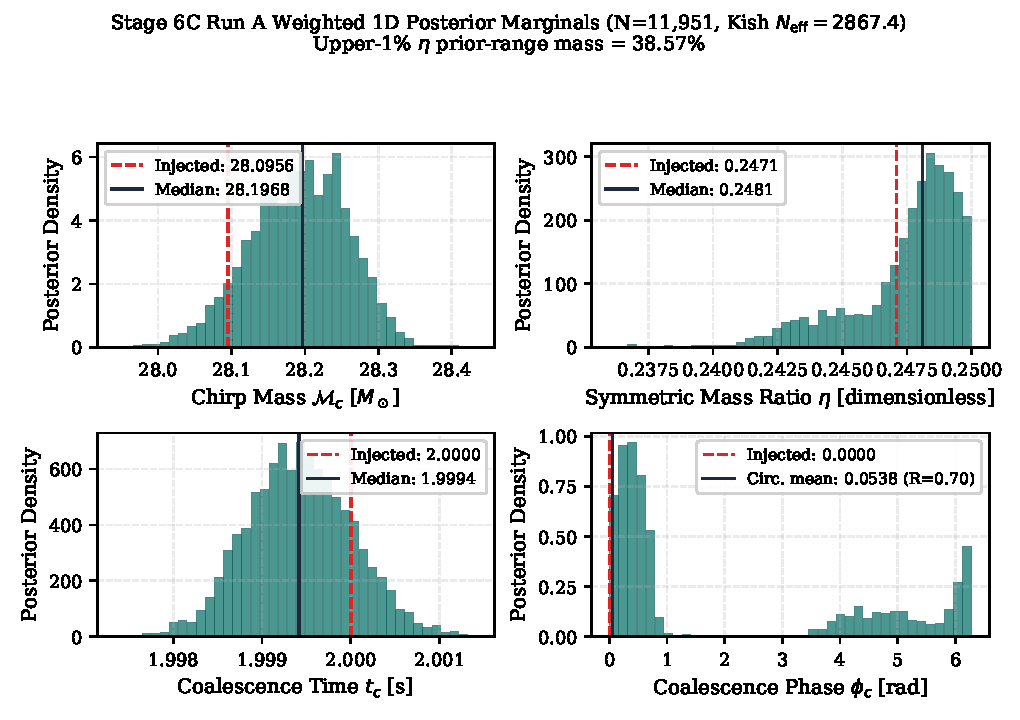
\includegraphics[width=0.95\textwidth]{figures/fig3_posterior_marginals.pdf}
    \caption{Weighted 1D marginal posterior densities from the saved synthetic benchmark posterior (random seed $8101$, $N=11{,}951$, Kish $N_{\mathrm{eff}}=2867.4$). Dashed red lines mark injected values; solid dark lines mark medians for $(\mathcal{M}_c, \eta, t_c)$ and the circular mean ($\bar{\phi}_c = 0.0538\,\mathrm{rad}$, $\bar{R} = 0.6991$) for periodic $\phi_c$.}
    \label{fig:posteriors}
\end{figure}

\textbf{What Figure~\ref{fig:posteriors} demonstrates:} Chirp mass $\mathcal{M}_c$ ($28.1968\,M_\odot$, $90\%$ CI $[28.0786, 28.2951]\,M_\odot$) and coalescence time $t_c$ ($1.9994\,\mathrm{s}$, $90\%$ CI $[1.9985, 2.0004]\,\mathrm{s}$) are tightly localized around the injection. Symmetric mass ratio $\eta$ exhibits strong accumulation against the physical equal-mass boundary $\eta = 0.25$: $38.57\%$ of posterior probability mass lies in the upper $1\%$ of the $\eta$ prior range ($\eta \ge 0.2485$). Coalescence phase $\phi_c$ wraps smoothly across $0 \equiv 2\pi$ with circular mean $0.0538\,\mathrm{rad}$.

\textbf{What Figure~\ref{fig:posteriors} does not demonstrate:} Because it is a single-seed synthetic run under the custom analytical PSD proxy, it does not establish sampler convergence across seeds, frequentist posterior coverage, or real-detector performance.

\section{Two-Seed Evidence Sensitivity Comparison}
Figure~\ref{fig:two_seed} compares two independent-seed runs under identical model and synthetic data: seed $8101$ ($\ln Z = 201646.1413 \pm 0.2374\,\mathrm{nats}$) versus seed $8201$ ($\ln Z = 201643.1693 \pm 0.2338\,\mathrm{nats}$). The observed difference is $|\Delta \ln Z| = 2.9720\,\mathrm{nats}$ with quadrature-combined internal uncertainty $\sigma_\Delta = 0.3332\,\mathrm{nats}$, yielding a discrepancy ratio of $8.92$.

\begin{figure}[H]
    \centering
    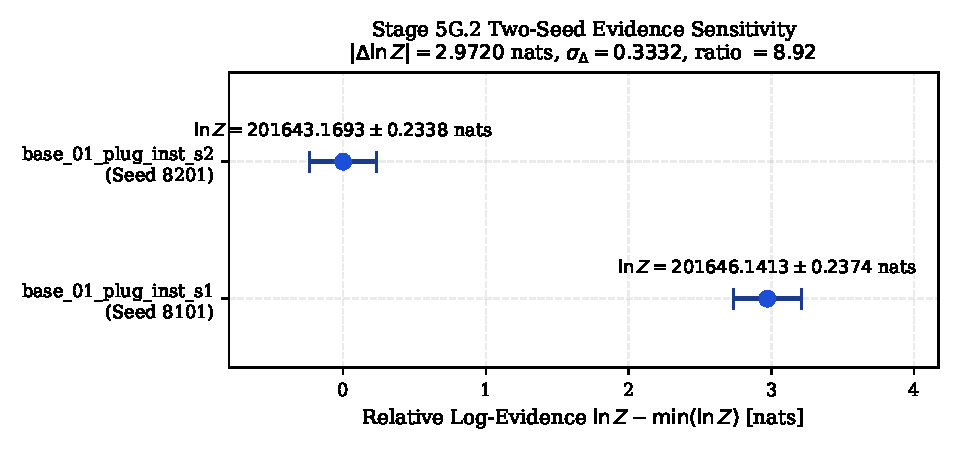
\includegraphics[width=0.88\textwidth]{figures/fig4_two_seed_evidence.pdf}
    \caption{Two-seed evidence sensitivity comparison (random seed $8101$ vs.\ $8201$ under identical synthetic data and Model~2 likelihood). The $2.9720\,\mathrm{nat}$ difference (ratio $8.92$) is a sensitivity diagnostic, not a convergence or coverage proof.}
    \label{fig:two_seed}
\end{figure}

\textbf{Qualification:} This ratio reflects internal sampler uncertainty reporting under $1$ degree of freedom; it is a sensitivity diagnostic, \emph{not} a calibrated frequentist significance, convergence proof, or coverage validation. Additional proposed runs (Run~B and seed~$8301$) remain unexecuted.

%==============================================================================
\chapter{Validation on Public GWOSC Detector Data}
%==============================================================================

\section{Real Strain Data and Validation Scope Separation}
GWLab separates three distinct verification tiers:
\begin{enumerate}[leftmargin=1.5em]
    \item \textbf{Synthetic software tests ($517/517$):} Validate internal mathematical consistency, Fourier/PSD conventions, and API contracts on synthetic data and saved archives.
    \item \textbf{Known-event external-data validation (this chapter):} Exercises conditioning, off-source Welch PSD estimation, and \texttt{gw\_inference.filter.matched\_filter} on public GWOSC \textbf{GW150914} (\texttt{GWTC-1-confident}, catalog GPS $1126259462.4$) via \path{scripts/validate_gw150914_gwosc.py}.
    \item \textbf{Full parameter-estimation and generalization validation:} Bayesian inference on real interferometer strain and multi-event blind searches have \emph{not} been performed.
\end{enumerate}

\section{Public Data Selection, Integrity, and Quality Flags}
Two official $32\,\mathrm{s}$, $4096\,\mathrm{Hz}$ HDF5 strain files starting at GPS $1126259447$ (UTC \texttt{2015-09-14T09:50:30}) were retrieved from the GWOSC v3 event API (\texttt{GW150914-v3}, catalog \texttt{GWTC-1-confident}), confirming use of a corrected release ($\ge\mathrm{v2}$) after the \texttt{v1} $4\,\mathrm{kHz}$ phase-error fix:
\begin{itemize}[leftmargin=1.5em]
    \item \textbf{H1:} \path{H-H1_GWOSC_4KHZ_R1-1126259447-32.hdf5} ($1{,}040{,}781\,\mathrm{bytes}$, $131{,}072$ finite samples, \texttt{DQmask = 127}, \texttt{Injmask = 31}), URL: \path{https://gwosc.org/eventapi/json/GWTC-1-confident/GW150914/v3/H-H1_GWOSC_4KHZ_R1-1126259447-32.hdf5}, SHA-256: \path{c5ea87beced5094b56b4d694f3a36e6d59f74d3a46e546b980a6a199d1f252a9}.
    \item \textbf{L1:} \path{L-L1_GWOSC_4KHZ_R1-1126259447-32.hdf5} ($1{,}007{,}262\,\mathrm{bytes}$, $131{,}072$ finite samples, \texttt{DQmask = 127}, \texttt{Injmask = 23}), URL: \path{https://gwosc.org/eventapi/json/GWTC-1-confident/GW150914/v3/L-L1_GWOSC_4KHZ_R1-1126259447-32.hdf5}, SHA-256: \path{9d65bde82f7ec035bea4c02228bce4acb3dcaae774c047edce71ef2ad64f1cc4}.
\end{itemize}
Inside the HDF5 \texttt{quality/simple} group, \texttt{DQmask = 127} ($0\mathrm{b}1111111$) verifies that all seven data-quality bits (\texttt{DATA}, \texttt{CBC\_CAT1}, \texttt{CBC\_CAT2}, \texttt{CBC\_CAT3}, \texttt{BURST\_CAT1}, \texttt{BURST\_CAT2}, \texttt{BURST\_CAT3}) pass for every second of the $32\,\mathrm{s}$ file. In \texttt{quality/injections}, \texttt{Injmask = 31} for H1 confirms all five \texttt{NO\_*\_HW\_INJ} flags pass, whereas \texttt{Injmask = 23} for L1 has bit~3 (\texttt{NO\_CW\_HW\_INJ}) equal to $0$: the L1 segment is \textbf{not injection-free} because O1 continuous-wave (CW) pulsar hardware injections were active (including O1 Pulsar~5 at $f_0 \approx 52.81\,\mathrm{Hz}$ inside the $[20, 67.65]\,\mathrm{Hz}$ template support, as well as higher-frequency lines at $108.86$, $145.2$--$145.4$, $194.31$, and $265.58\,\mathrm{Hz}$). In the $4.0\,\mathrm{s}$ ($\Delta f = 0.25\,\mathrm{Hz}$) L1 off-source Welch PSD, the $[52.5, 53.0]\,\mathrm{Hz}$ power ratio to the local $50$--$55\,\mathrm{Hz}$ median is $1.18$, showing no detectable line excess above the noise floor at this resolution, while the L1 result remains explicitly qualified for active CW hardware-injection flags. The validation script checks \texttt{(dq\_mask \& 0b0001111) == 0b0001111} and \texttt{(inj\_mask \& 0b00011) == 0b00011}.

\section{Conditioning and Off-Source Welch PSD Estimation}
Raw interferometer strain exhibits strong sub-$15\,\mathrm{Hz}$ seismic drift and non-zero DC offsets (for example, L1 raw strain spans $[-1.87, -0.046]\times 10^{-18}$). Each $32\,\mathrm{s}$ time series is conditioned by: (1) subtracting the full-stretch mean; (2) applying a zero-phase $4$th-order Butterworth high-pass filter at $15\,\mathrm{Hz}$; and (3) applying polyphase FIR anti-alias filtering and downsampling from $4096\,\mathrm{Hz}$ to $2048\,\mathrm{Hz}$ ($65{,}536$ samples). Filter edge regions ($[0, 1]\,\mathrm{s}$ and $[31, 32]\,\mathrm{s}$) are excluded from all subsequent analysis. Figure~\ref{fig:gw150914_strain} shows the conditioned strain around the event.

To avoid fitting the event signal itself, the PSD is estimated strictly from off-source intervals $[1, 13]\,\mathrm{s}$ (pre-event) and $[18, 30]\,\mathrm{s}$ (post-event), excluding a $5\,\mathrm{s}$ guard around $t_{\mathrm{rel}} = 15.4\,\mathrm{s}$, using \texttt{gw\_inference.psd.welch\_psd} with $4.0\,\mathrm{s}$ Tukey-windowed ($\alpha=0.25$) segments at $50\%$ overlap. Figure~\ref{fig:gw150914_psd} shows the resulting off-source ASDs, highlighting narrowband instrumental lines ($60\,\mathrm{Hz}$ mains, violin modes near $300\,\mathrm{Hz}$) and the steep low-frequency seismic wall absent from the smooth synthetic \texttt{aligo\_representative} proxy. Whitening the $[25, 350]\,\mathrm{Hz}$ band clearly reveals the GW150914 chirp pulse in both detectors (Figure~\ref{fig:gw150914_whitened}).

\begin{figure}[H]
    \centering
    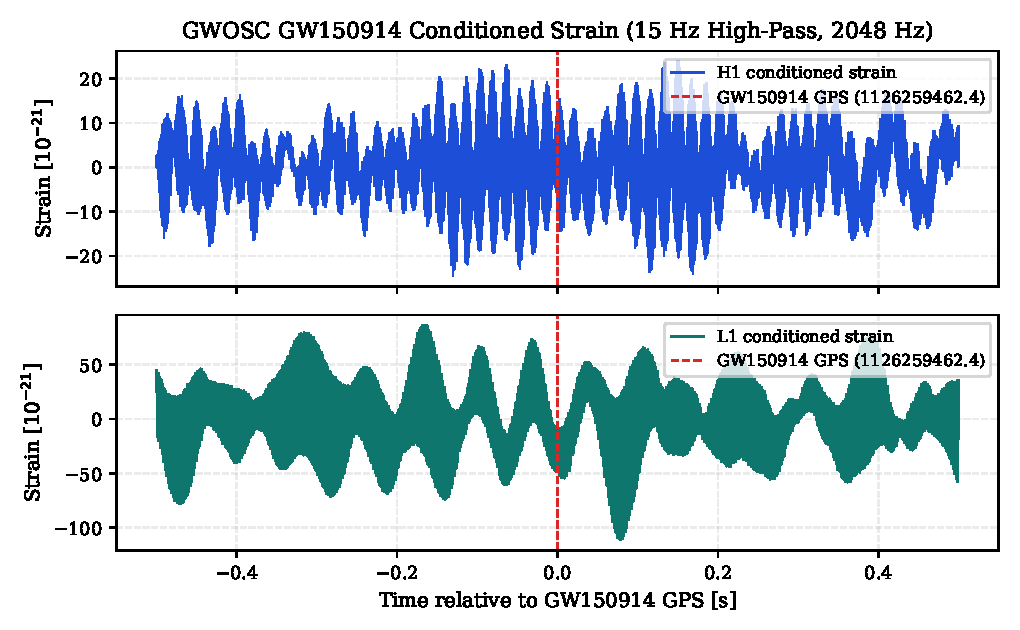
\includegraphics[width=0.92\textwidth]{figures/gw150914_external/fig_gw150914_strain.pdf}
    \caption{Conditioned H1 and L1 GWOSC strain ($15\,\mathrm{Hz}$ high-pass, $2048\,\mathrm{Hz}$) around GW150914 (GPS $1126259462.4$).}
    \label{fig:gw150914_strain}
\end{figure}

\begin{figure}[H]
    \centering
    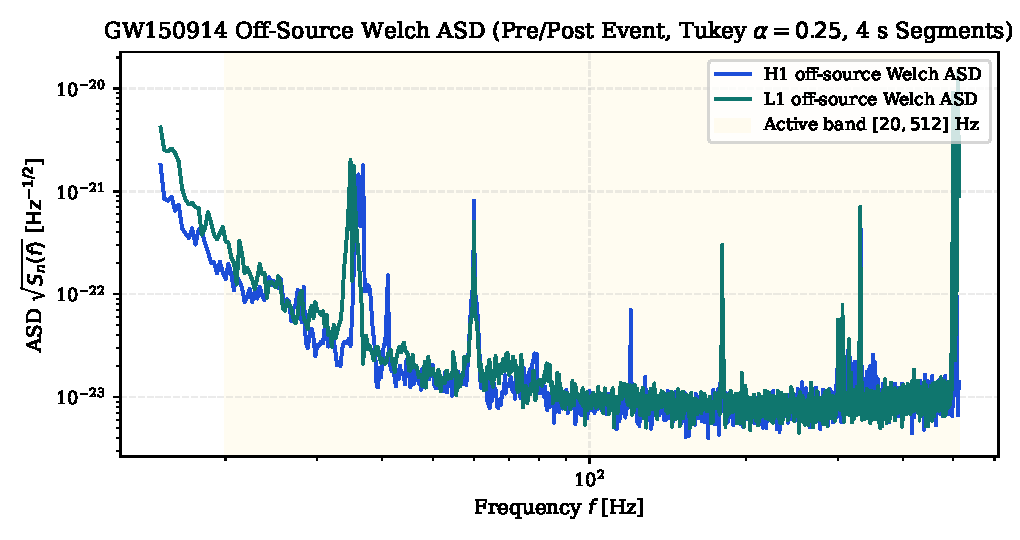
\includegraphics[width=0.92\textwidth]{figures/gw150914_external/fig_gw150914_psd_asd.pdf}
    \caption{Off-source Welch ASDs $\sqrt{S_n(f)}$ for H1 and L1 estimated strictly outside the GW150914 event window, showing real O1 spectral lines and low-frequency seismic noise.}
    \label{fig:gw150914_psd}
\end{figure}

\begin{figure}[H]
    \centering
    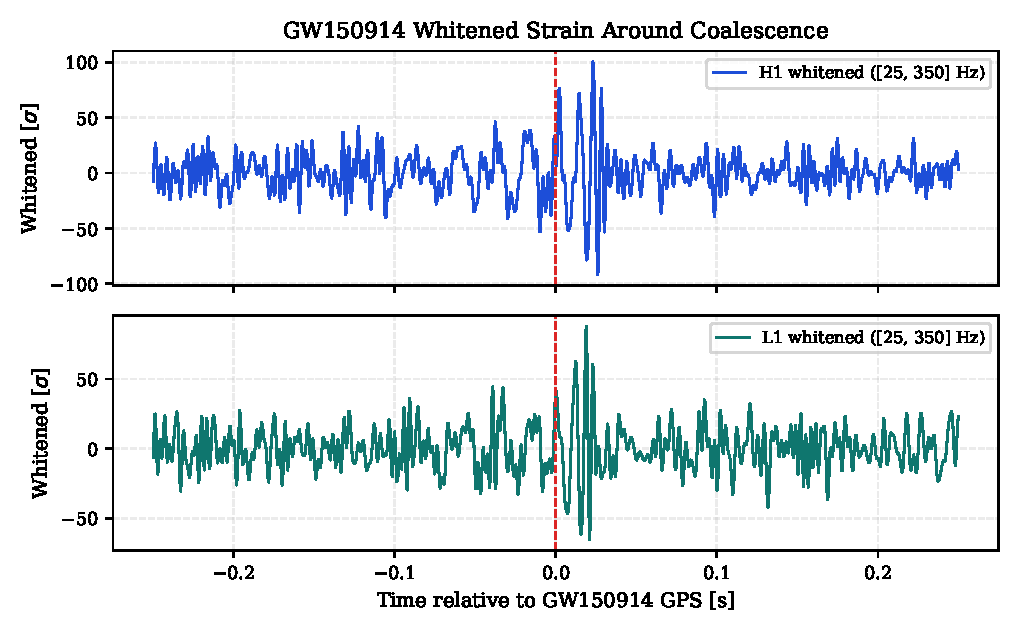
\includegraphics[width=0.92\textwidth]{figures/gw150914_external/fig_gw150914_whitened.pdf}
    \caption{Whitened H1 and L1 strain ($[25, 350]\,\mathrm{Hz}$) revealing the coherent GW150914 chirp waveform near $t_{\mathrm{rel}} = 0\,\mathrm{s}$.}
    \label{fig:gw150914_whitened}
\end{figure}

\section{Matched-Filter Search, Results, and TaylorF2 Limitations}
A fixed, non-optimized inspiral template applied to a known event (\texttt{TaylorF2}, $m_1 = 35.0\,M_\odot$, $m_2 = 30.0\,M_\odot$, $\mathcal{M}_c = 28.19\,M_\odot$, $\eta = 0.2485$, $f_{\mathrm{ISCO}} = 67.65\,\mathrm{Hz}$) was evaluated over $[20, 512]\,\mathrm{Hz}$ on a $4.0\,\mathrm{s}$ Tukey-windowed ($\alpha=0.1$) on-source segment centered on GW150914 using \texttt{gw\_inference.filter.matched\_filter}.

As shown in Figures~\ref{fig:gw150914_snr} and~\ref{fig:gw150914_comp}, this fixed, non-optimized inspiral template recovers coherent SNR peaks in both detectors:
\begin{itemize}[leftmargin=1.5em]
    \item \textbf{LIGO Hanford (H1):} Peak SNR $|\rho| = 8.94$ at $+71.8\,\mathrm{ms}$ relative to catalog GPS ($1126259462.4718$).
    \item \textbf{LIGO Livingston (L1):} Peak SNR $|\rho| = 5.55$ at $+61.0\,\mathrm{ms}$ relative to catalog GPS ($1126259462.4610$).
\end{itemize}
Both peaks align within the physical $\sim 10\,\mathrm{ms}$ inter-site light-travel window. Crucially, the recovered inspiral SNRs ($8.94$ and $5.55$) are smaller than LIGO's full inspiral--merger--ringdown (IMR) network SNR ($\sim 24$) because \texttt{TaylorF2} terminates at $f_{\mathrm{ISCO}} = 67.65\,\mathrm{Hz}$: for a $\sim 65\,M_\odot$ binary in O1 noise, most signal power in the sensitive $[68, 250]\,\mathrm{Hz}$ band comes from the plunge, merger, and ringdown omitted by a nonspinning inspiral-only approximant.

\begin{figure}[H]
    \centering
    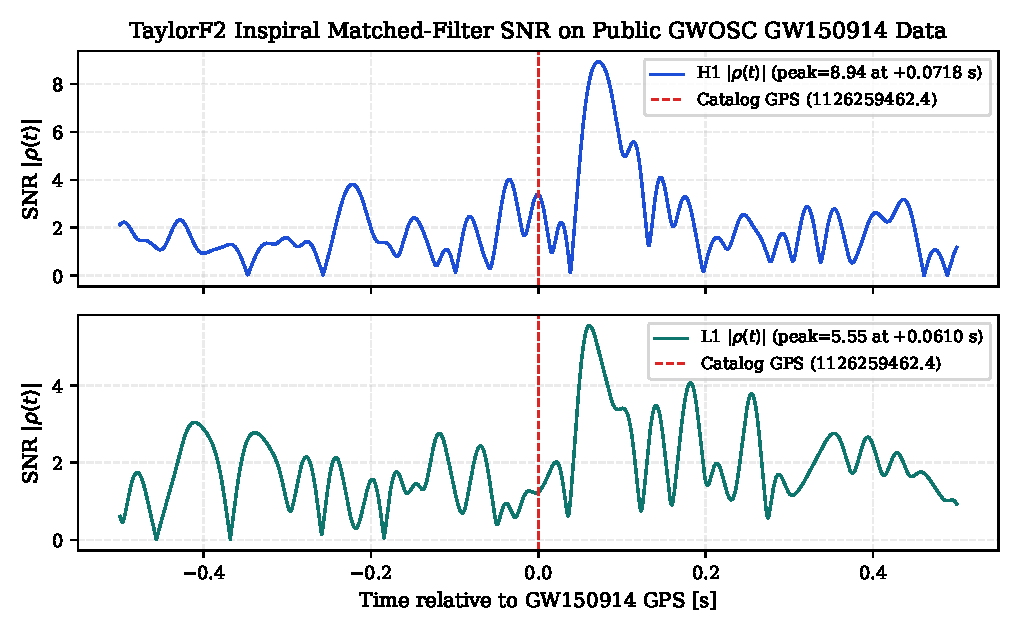
\includegraphics[width=0.92\textwidth]{figures/gw150914_external/fig_gw150914_snr.pdf}
    \caption{Matched-filter SNR $|\rho(t)|$ on public GWOSC GW150914 data using a fixed, non-optimized \texttt{TaylorF2} inspiral template ($35 + 30\,M_\odot$, $f_{\mathrm{ISCO}} = 67.65\,\mathrm{Hz}$) applied to a known event.}
    \label{fig:gw150914_snr}
\end{figure}

\begin{figure}[H]
    \centering
    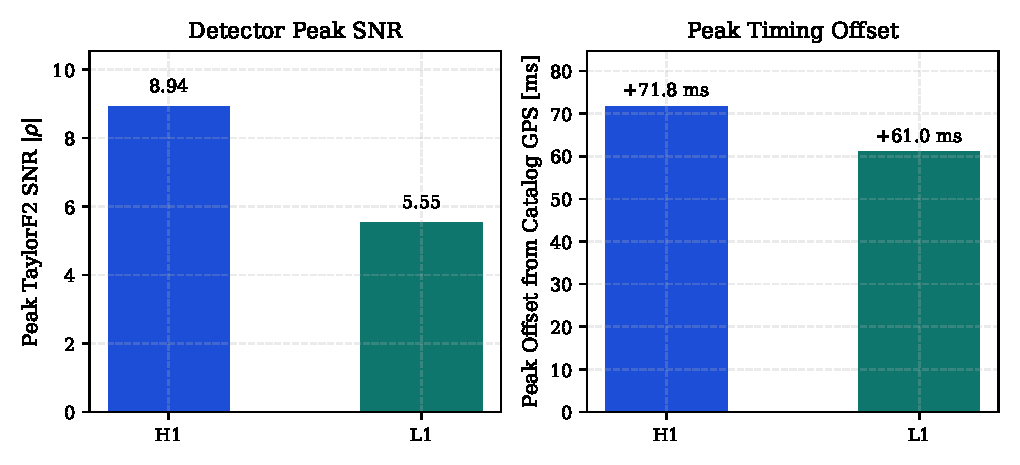
\includegraphics[width=0.90\textwidth]{figures/gw150914_external/fig_gw150914_detector_comparison.pdf}
    \caption{Comparison of H1 and L1 peak \texttt{TaylorF2} inspiral SNR and timing offset relative to the GW150914 catalog GPS.}
    \label{fig:gw150914_comp}
\end{figure}

\section{Data Acknowledgement}
This validation uses data obtained from the Gravitational Wave Open Science Center (\url{https://gwosc.org}), a service of LIGO Laboratory, the LIGO Scientific Collaboration, and the Virgo Collaboration. LIGO was constructed by the California Institute of Technology and Massachusetts Institute of Technology with funding from the National Science Foundation.

%==============================================================================
\chapter{Validation, Reproducibility, and Deployment Status}
%==============================================================================

Table~\ref{tab:validation_summary} summarizes the verification status across the backend, frontend, and packaging layers. All interactive calculations are deterministic for fixed seeds (`7101` off-source noise, `7151` on-source matched filter), and all archived results are traced in Appendix~\ref{app:provenance}.

\begin{table}[H]
    \centering
    \caption{System Validation and Release-Readiness Summary.}
    \label{tab:validation_summary}
    \small
    \begin{tabular}{p{4.3cm}p{3.4cm}p{7.2cm}}
        \toprule
        \textbf{Layer / Check} & \textbf{Verified Result} & \textbf{Scope \& Notes} \\
        \midrule
        Full Repository \texttt{pytest} & $517/517$ passing & All physics, likelihood, sampler, and API tests \\
        GWLab Backend \& Config Tests & $62/62$ passing & \texttt{tests/test\_gwlab\_*.py} \\
        \texttt{src/gwlab/} Coverage & $86\%$ ($788/911$ stmts) & Exceeds $85\%$ target \\
        Playwright E2E Matrix & $21/21$ passing & $7$ routes $\times$ $3$ viewports; $0$ errors/overflows \\
        TypeScript / ESLint / Build & $0$ errors & \texttt{standalone} build verified; $7$ lint warnings \\
        Local Launcher Preflight & Passed & Checks deps, artifacts, build, and ports \\
        Docker Build / Compose Run & Not executed locally & Configured; \texttt{docker} CLI absent on host \\
        Offline Font Serving & Runtime self-hosted & $50$ \texttt{.woff2} bundled; build fetches Google Fonts \\
        \bottomrule
    \end{tabular}
\end{table}

%==============================================================================
\chapter{Limitations, Conclusion, and Future Work}
%==============================================================================

\section{Scientific and Operational Limitations}
\begin{enumerate}[leftmargin=1.5em]
    \item Interactive pages use synthetic data and the custom \texttt{aligo\_representative} PSD proxy rather than official LIGO sensitivity curves or open strain data.
    \item The Bayesian posterior explorer reflects a single-seed archived run (`8101`), and the two-seed comparison (`8101` vs.\ `8201`) is a sensitivity diagnostic only.
    \item Proposed extensions (Run~B, seed~$8301$) remain unexecuted, and Model~3 (Student-$t$ likelihood) remains frozen/specified and unapproved for production inference.
    \item Docker Compose execution on a Docker-enabled host and fully offline clean `next build` font bundling remain external validation steps.
\end{enumerate}

\section{Conclusion}
GWLab delivers a unified, mathematically audited gravitational-wave analysis laboratory connecting post-Newtonian waveform physics, colored-noise Welch estimation, matched filtering, normalized Whittle likelihoods, and nested-sampling posterior forensics within a validated Next.js + FastAPI architecture, supplemented by reproducible external validation on public GWOSC GW150914 detector strain.

\appendix

%==============================================================================
\chapter{Notation, Parameters, and Provenance}\label{app:provenance}
%==============================================================================

\section{Notation and Physical Constants}
\begin{table}[H]
    \centering
    \caption{Core Symbols, Physical Constants, and SI Units.}
    \small
    \begin{tabular}{p{3.0cm}p{5.0cm}p{6.8cm}}
        \toprule
        \textbf{Symbol} & \textbf{Meaning} & \textbf{Value / Units} \\
        \midrule
        $c, G$ & Speed of light, gravitational constant & $299{,}792{,}458\,\mathrm{m\,s^{-1}}$, $6.67430\times 10^{-11}\,\mathrm{m^3\,kg^{-1}\,s^{-2}}$ \\
        $M_\odot, C_{\mathrm{ISCO}}$ & Solar mass, Schwarzschild ISCO constant & $1.9884099\times 10^{30}\,\mathrm{kg}$, $4397.17\,\mathrm{Hz}\cdot M_\odot$ \\
        $\mathcal{M}_c, \eta, M$ & Chirp mass, symmetric mass ratio, total mass & $M_\odot$, dimensionless $(0, 0.25]$, $M_\odot$ \\
        $S_n(f), \sqrt{S_n(f)}$ & One-sided PSD, Amplitude Spectral Density & $\mathrm{Hz}^{-1}$, $\mathrm{Hz}^{-1/2}$ \\
        $\rho(t), \rho_{\mathrm{opt}}$ & Complex matched-filter SNR, optimal SNR & Dimensionless \\
        $\ln Z, N_{\mathrm{eff}}$ & Log-Bayesian evidence, Kish effective sample size & $\mathrm{nats}$, dimensionless \\
        \bottomrule
    \end{tabular}
\end{table}

\section{Benchmark Parameters and Sampler Configuration}
\begin{table}[H]
    \centering
    \caption{Frozen Reference Benchmark and Sampler Configuration.}
    \small
    \begin{tabular}{p{4.3cm}p{5.5cm}p{5.0cm}}
        \toprule
        \textbf{Parameter / Setting} & \textbf{Value} & \textbf{Units / Notes} \\
        \midrule
        Duration $T$ / Rate $f_s$ & $4.0$ / $2048.0$ & $\mathrm{s}$ / $\mathrm{Hz}$ ($N=8192$, $\Delta f = 0.25\,\mathrm{Hz}$) \\
        Active frequency band & $[20.0, 512.0]$ & $\mathrm{Hz}$ ($\mathcal{K}_+$ static mask) \\
        Injected $(\mathcal{M}_c, \eta, d_L, t_c, \phi_c)$ & $(28.0956, 0.2471, 410.0, 2.0, 0.0)$ & $M_\odot$, $-$, $\mathrm{Mpc}$, $\mathrm{s}$, $\mathrm{rad}$ \\
        4D Uniform Prior Support & $[20,40]\times[0.10,0.25]\times[1.9,2.1]\times[0,2\pi)$ & Direct $(\mathcal{M}_c, \eta, t_c, \phi_c)$ measure \\
        Sampler (\texttt{dynesty}) & $N_{\mathrm{live}}=500$, \texttt{multi}, \texttt{rwalk}, $\Delta\ln Z=0.10$ & Random seed $8101$ \\
        \bottomrule
    \end{tabular}
\end{table}

\section{Archive Provenance Mapping}
\begin{table}[H]
    \centering
    \caption{Mapping Between Monograph Descriptions and Internal Archive Identifiers.}
    \small
    \begin{tabular}{p{3.9cm}p{3.6cm}p{7.4cm}}
        \toprule
        \textbf{Monograph Term} & \textbf{Internal ID} & \textbf{Repository Artifact Path} \\
        \midrule
        Saved benchmark posterior & Stage 6C Run A (\texttt{run\_a\_anchor}) & \path{experiments/wp6_stage6c_anchor/run_a_anchor_samples.npz} \\
        Benchmark summary JSON & Stage 6C Run A result & \path{experiments/wp6_stage6c_anchor/run_a_anchor_result.json} \\
        Two-seed sensitivity pair & Stage 5G.2 (\texttt{s1} vs \texttt{s2}) & \path{reports/demonstrations/wp6_stage5/stage_g2/} \\
        Historical resource ledger & Stage 6D ledger & \path{experiments/wp6_stage6c_anchor/stage6c_aggregate_ledger.json} \\
        \bottomrule
    \end{tabular}
\end{table}

\begin{thebibliography}{9}
\bibitem{SathyaprakashDhurandhar1991}
B.~S. Sathyaprakash and S.~V. Dhurandhar, ``Choice of filters for the detection of gravitational waves from coalescing binaries,'' \emph{Phys. Rev. D}, vol.~44, pp.~3819--3834, 1991.

\bibitem{Finn1992}
L.~S. Finn, ``Detection, measurement, and gravitational radiation,'' \emph{Phys. Rev. D}, vol.~46, pp.~5236--5249, 1992.

\bibitem{CutlerFlanagan1994}
C.~Cutler and E.~E. Flanagan, ``Gravitational waves from merging compact binaries: How accurately can one extract the binary's parameters from the inspiral waveform?,'' \emph{Phys. Rev. D}, vol.~49, pp.~2658--2697, 1994.

\bibitem{Buonanno2009}
A.~Buonanno, B.~R. Iyer, E.~Ochsner, Y.~Pan, and B.~S. Sathyaprakash, ``Comparison of post-Newtonian templates for compact binary inspiral signals in gravitational-wave detectors,'' \emph{Phys. Rev. D}, vol.~80, p.~084043, 2009.

\bibitem{Allen2012}
B.~Allen, W.~G. Anderson, P.~R. Brady, D.~A. Brown, and J.~D.~E. Creighton, ``FINDCHIRP: An algorithm for detection of gravitational waves from inspiraling compact binaries,'' \emph{Phys. Rev. D}, vol.~85, p.~122006, 2012.

\bibitem{Welch1967}
P.~D. Welch, ``The use of fast Fourier transform for the estimation of power spectra: A method based on time averaging over short, modified periodograms,'' \emph{IEEE Trans. Audio Electroacoust.}, vol.~15, no.~2, pp.~70--73, 1967.

\bibitem{Skilling2006}
J.~Skilling, ``Nested sampling for general Bayesian computation,'' \emph{Bayesian Analysis}, vol.~1, no.~4, pp.~833--859, 2006.

\bibitem{Speagle2020}
J.~S. Speagle, ``\texttt{dynesty}: a dynamic nested sampling package for estimating Bayesian posteriors and evidences,'' \emph{Mon. Not. R. Astron. Soc.}, vol.~493, no.~3, pp.~3132--3158, 2020.
\end{thebibliography}

\end{document}
